\subsection{Convolutional Neural Network}

\begin{frame}
\frametitle{Biologische Zellarten}

\begin{figure}
	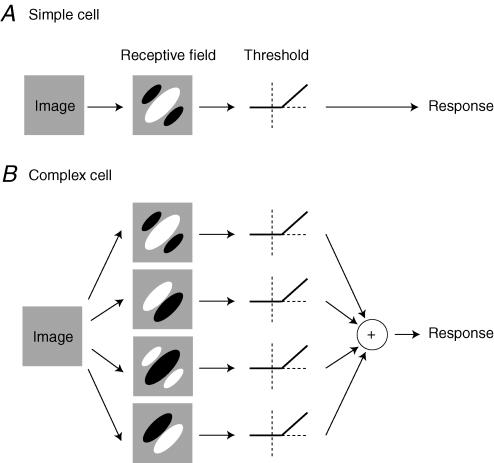
\includegraphics[width=.7\linewidth]{./aktuelleEntwicklung/convolutionalNN/img/simpleVsComplex_alpha}
\end{figure}


\note[item]{1962: zwei Neurophysiologen Torsten Wiesel und David Hubel}

\note[item]{Konzept der simple und complex cells
\begin{itemize}
    \item nicht positionsbunden - spatial invariance, räumliche Invarianz
\end{itemize}}

\note[item]{Arten von Zellen zur Erkennung einfacher Kanten und Balken
\begin{itemize}
    \item \emph{simple cells}: ist Positionsgebunden
    \item \emph{complex cells}: Muster können an beliebigen Positionen auftauchen
\end{itemize}}

\note[item]{1962: Konzept wie im Bild}
\note[item]{1980er Dr. Kunihiko Fukushima: erstes Modell nach diesem Konzept}

\end{frame}


\begin{frame}
\frametitle{Convolutinal Layer - Filter}

\begin{itemize}
\item Mehrdimensionales Array mit Farbwerten zur Repräsentation im Rechner
\item Durch Filter auf bestimmte \emph{Low-Level} Eigenschaften schließen
\end{itemize}

\begin{figure}
	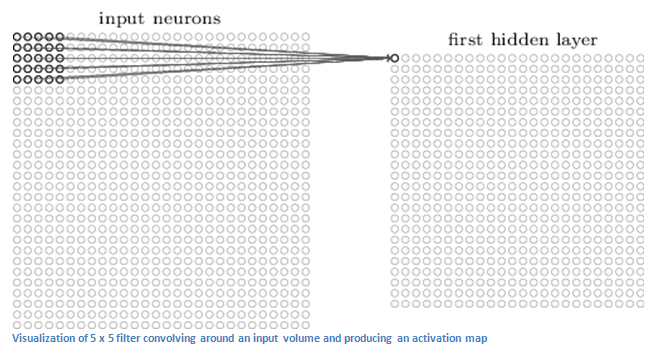
\includegraphics[width=.8\linewidth]{./aktuelleEntwicklung/convolutionalNN/img/cnn_convLayer_alpha}
\end{figure}


\note[item]{Array als Eingabe
\begin{itemize}
    \item Repräsentiert die Pixel im Bild
\end{itemize}}

\note[item]{Farbwertearray kann pro Pixel mehrere Werte enthalten
\begin{itemize}
    \item entsprechend eventuell auch mehrere Dimensionen im Array
\end{itemize}}

\note[item]{Fenster \emph{läuft} Eingabematrix ab
\begin{itemize}
    \item dadurch simple Formen erkennen
    \item Beispiel folgt
\end{itemize}}

\note[item]{Hidden Layer kann als Ansammlung von low-level Merkmalen verstanden werden}

\end{frame}


\begin{frame}
\frametitle{Filter - Funktionsweise}

\begin{figure}
	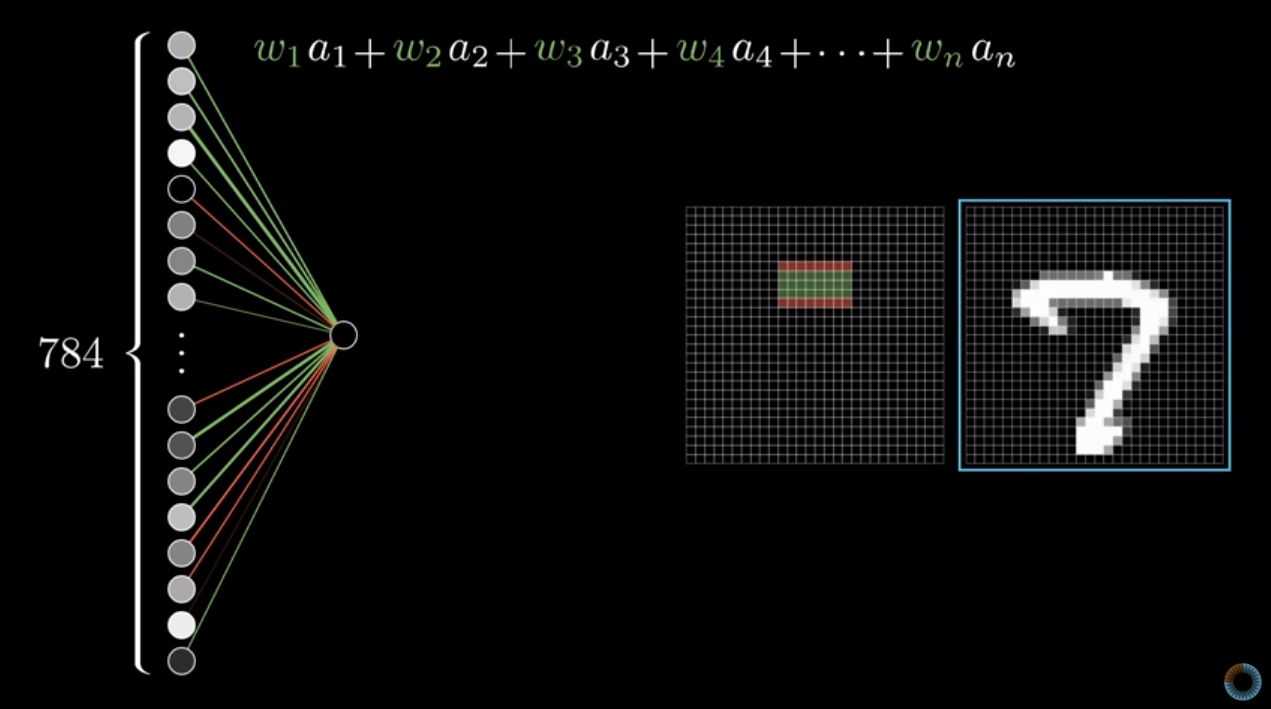
\includegraphics[width=\linewidth]{./aktuelleEntwicklung/convolutionalNN/img/filter}
\end{figure}

\note[item]{Bild erläutern
\begin{itemize}
    \item Beispiel: Ziffer 7
    \item Strich am oberen Rand
    \item Gewichtsmatrix hier getrennt aufgeführt
    \item rot: negative Werte
    \item grün: positive Werte
\end{itemize}}

\note[item]{Dieses Feature (oberer Strich) kann aber auch bei anderen Ziffern auftauchen
\begin{itemize}
    \item Bsp. schlecht geschriebene Ziffer Null
\end{itemize}}

\note[item]{Erkannte Merkmale können von weiteren Filtern genutzt werden
\begin{itemize}
    \item erinnert an ganz alte Prinzipien 
    \item wie schonn beim Adeline Modell, hier jedoch mit mehreren Schichten
\end{itemize}}

\end{frame}


\begin{frame}
\frametitle{Pooling Layer}

\begin{itemize}
\item Aggregiert die Ergebnisse von Convolutional Layern
\item Ziele
\begin{itemize}
	\item Nur die relevantesten Signale an nächste Schicht weitergeben
	\item Anzahl der Parameter im Netz reduzieren
\end{itemize}

\item \emph{MaxPooling Layer} am weitesten verbreitet
\end{itemize}



\note[item]{Pooling Layer
\begin{itemize}
    \item aggregiert Ergebnisse von Convolutional Layern
    \item Zweck: nur die relevantesten Signale an die nächste Schicht weitergeben 
\end{itemize}}

\note[item]{\emph{während die Größe des Inputs durch die Faltungen und das Pooling immer weiter reduziert wird, erhöht sich die Anzahl der Filter zur Erkennung von übergeordneten Signalen zunehmend}}

\note[item]{Verschiedene Pooling-Mechanismen:
\begin{itemize}
    \item MaxPooling: 
    \begin{itemize}
        \item am weitesten verbreitet
        \item maximale Eingabewert wird weitergegeben
    \end{itemize}
    \item fractional max pooling
    \item lp pooling
    \item mean pooling
    \item stochastic pooling 
    \item spatial pooling
    \item generalized pooling
\end{itemize}}

\end{frame}



\begin{frame}
\frametitle{Fully Connected Layer}

\begin{itemize}
\item Ausgangspunkt: \emph{High-Level} Merkmale bereits durch frühere Schichten erkannt 
\item Alle Neuronen der Ausgabeschicht sowie dieser Merkmale direkt miteinander verbunden
\item Ausgabe sollte mit den richtigen Gewichten / Schwellwerten relativ eindeutige Ausgaben generieren
\end{itemize}

\begin{figure}
	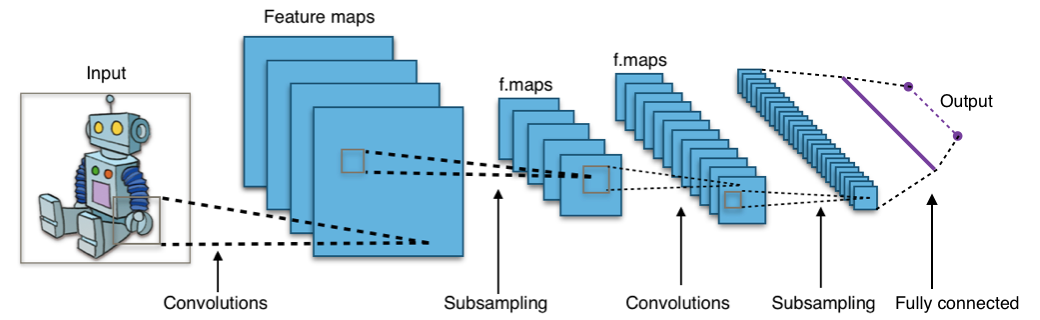
\includegraphics[width=.9\linewidth]{./aktuelleEntwicklung/convolutionalNN/img/cnn_overview_alpha}
\end{figure}


\note[item]{auch \emph{dense Layer} genannt}
\note[item]{Ausgagngspunkt: \emph{High-Level} Merkmale bereits durch frühere Schichten erkannt
\begin{itemize}
    \item Neuronen halten diese Eigenschaften
\end{itemize}}

\note[item]{Ausgabeneuronen repräsentieren verschienden Klassen
\begin{itemize}
    \item siehe Klassifizierungsproblem
    \item Fully connected Layer: stellt verbindung zwischen letztem hidden Layer und Ausgabelayer bereit
\end{itemize}}

\note[item]{Beispiel: Schnörkel zu Ziffern interpretieren
\begin{itemize}
    \item 10 dimensionaler Ausgabevektor bei Ziffern
\end{itemize}}

\end{frame}

